\documentclass[a4paper,10pt, twoside]{article}
\usepackage[utf8]{inputenc}
\setcounter{tocdepth}{2} %Only show sections and subsections in toc.

\usepackage{colortbl}
\usepackage{siunitx} %Package for SI units
\sisetup{per-mode=fraction}

\usepackage{textcomp} %Vertically centered tilde (~)
\usepackage{amsmath}
\usepackage{graphicx}
\usepackage{standalone}

\usepackage[font={footnotesize}]{caption}
\usepackage[font={footnotesize}]{subcaption}

\usepackage[hidelinks]{hyperref}
%\hypersetup{
%    colorlinks = false,
%    linkbordercolor = {white},
%}


%\hypersetup{
 %   colorlinks,
 %   linkcolor={red!50!black},
 %   citecolor={blue!50!black},
 %   urlcolor={blue!80!black}
%}

\usepackage{float}
\usepackage[procnames]{listings}
\usepackage{epstopdf} %Convert EPS files to PDF format
\usepackage{pdfpages} %Utility to include pdf documents into the report, used to include datasheets in appendices.

\usepackage{tikz} 			%Utility to draw nice figures
\usetikzlibrary{shapes.geometric, arrows}
\usepackage{standalone}
\usepackage{circuitikz} 	%Utility to draw circuits in tikz

\usepackage[disable]{todonotes}
\usepackage{listings}
\usepackage{multirow}


\usepackage{url}
\renewcommand{\UrlFont}{\large\tt}

\usepackage{chngcntr} %Change the counters of objects. Used to make figure/table and equation counting specific to the section they are in.
\counterwithin{figure}{section}
\counterwithin{equation}{section}

%Make counter of listings specific to sections
\AtBeginDocument{%
  \counterwithin*{lstlisting}{section}
  \renewcommand{\thelstlisting}{%
    \ifnum\value{subsection}=0
      \thesection.\arabic{lstlisting}%
    \else
      \ifnum\value{subsubsection}=0
        \thesection.\arabic{lstlisting}%
      \else
        \thesection.\arabic{lstlisting}%
      \fi
    \fi
  }%
}

\usepackage[inner=2cm,outer=4cm]{geometry}



\setlength{\parindent}{0pt}

\title{Electronics - 1. Semester Project}
\author{Thomas Søndergaard Christensen, Erlingur Ívar Jóhannsson, Mikkel Skarup Jaedicke, Morten Tholstrup Pedersen, Martin Brøchner Andersen}
\date{31/05/2016}


\begin{document}
%!TEX root = ../main.tex
\begin{titlepage}
%\newgeometry{left=3cm,right=3cm}
\begin{center}

\textsc{\LARGE University of Southern Denmark}\\[1.5cm]
\textsc{\Large MSc in Engineering - Electronics}\\
\textsc{\large 2. Semester Project}\\[0.5cm]

\vfill
\vspace{3cm}
\hrule ~\\[0.3cm]
{ \LARGE \bfseries Monitoring System for the SDU Go-Kart\\[0.4cm] }
\hrule ~\\[1.5cm]

\vfill

%\includegraphics[width=0.3\textwidth]{graphics/sdu_logo}
\vspace{7cm}
% Author and supervisor
\begin{minipage}[t]{.55\textwidth}
\begin{flushleft} \large
\textbf{Authors:}\\
230390 Martin Brøchner Andersen\\
151088 Catalin Ionut Ntemkas\\
030192 Mikkel Skaarup Jaedicke\\
100589 Thomas S. Christensen
\end{flushleft}
\end{minipage}
\begin{minipage}[t]{.44\textwidth}
\begin{flushright} \large
\textbf{Supervisor:} \\
Leon Bonde Larsen
\end{flushright}
\end{minipage}

\vspace{1cm}
Date: 19-12-2016

\vspace{1cm}

\end{center}
%\restoregeometry
\end{titlepage}
\newpage
\pagenumbering{Roman}
%!TEX root = ../main.tex
\section*{Preface}
\addcontentsline{toc}{section}{Preface}

\section*{Acknowledgment}
\addcontentsline{toc}{section}{Acknowledgment}
This project would not have been possible without the invaluable assistance and patience of our supervisor. 
A Tremendous thank you to Leon Bonde Larsen.
The process was simplified by Assistant Professor Kjeld Jensen from which the sensory equipment used in the report was supplied.
\thomas{Rewritten - needs a bit more?}
\martin{Who else should we thank? Viking Pizza?}
\mikkel{NEW URL}
\vspace{5cm}
\begin{center}
	\begin{minipage}[t]{.55\textwidth}\large
		\begin{center}
		Catalin Ionut Ntemkas\\
		\vspace{1cm}
		\hrule
		\vspace{0.5cm}
		Martin Brøchner Andersen\\
		\vspace{1cm}
		\hrule
		\vspace{0.5cm}
		Mikkel Skaarup Jaedicke\\
		\vspace{1cm}
		\hrule
		\vspace{0.5cm}
		Thomas Søndergaard Christensen
		\vspace{1cm}
		\hrule
		\end{center} 
	\end{minipage}
\end{center}

\vspace{1.2cm}
  \begin{center}
    \textsl{The report, source code, data, plotting script and simulations can be found at:}  
    \end{center}
    \vspace{-5pt}
    \begin{center}
	\renewcommand{\UrlFont}{\color{black}\normalsize\tt}
    \url{github.com/mikkeljae/SEM1PRO_ELECTRONICS}
   \end{center}
\newpage

\section*{Abstract}
\addcontentsline{toc}{section}{Abstract}
A go-kart has been supplied as a development platform for student projects at University of Southern Denmark.
In the interest of enabling more complex projects, a unified data collection system is necessary.
This is developed throughout this report. 
An analysis is done to determine the requirements of such a system.
It was found that a two-part network is suitable for this application.
The two parts are a CAN network and an ad-hoc WiFi network.
A custom protocol for use on CAN, GoCAN, is developed.
GoCAN supports up to 16 sensors from which data can be monitored on a remote monitoring station using the WiFi connection.
The system was only partially implemented since a connection between the CAN network and Linux was not achieved.
\thomas{Rewritten}
\newpage
\tableofcontents
\newpage
\listoftodos
%\listoftables
\clearpage
\newpage
\pagenumbering{arabic}
%!TEX root = ../main.tex
\section{System Description}
\label{sec:system_description}
This project is aimed at developing a backbone for data collection on the SDU go-kart.
As mentioned, the go-kart is intended as a development platform to be used by students on the master's programme in electronics on SDU.
Some projects may implement new sensory equipment while others may work on improving the inverter.
Common for all of them is that they require access to the data that their system is producing.
Providing a unified structure for gathering data from the go-kart will greatly ease the development on the platform, especially across different projects with different developers.
A system will be developed which provides a simple method for accessing data wirelessly on the go-kart while driving.
Live access of parameters while driving, realistically, requires some form of wireless communication between a monitoring system and the go-kart, see figure \ref{fig:simple}.

\begin{figure}[h]
 	\centering
    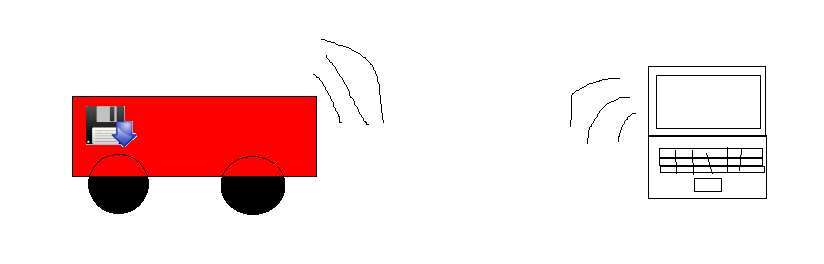
\includegraphics[width=0.6\textwidth]{graphics/go_kart_network_simple}
    \caption{SDU go-kart transferring data to a stationary computer wirelessly.}
    \label{fig:simple}
\end{figure}

While the system should be able to provide a live feed of the data being collected on the system, it should also log all data during a drive, with the possibility of transferring it later.
This will enable the user to do more advanced data analysis on the dataset than what can be achieved by monitoring the data.
In some cases, certain parameters may be irrelevant to the test being performed.
Transmitting these parameters should be avoidable by providing the possibility to start and stop data collection from specific data producers.

\begin{figure}[h]
 	\centering
    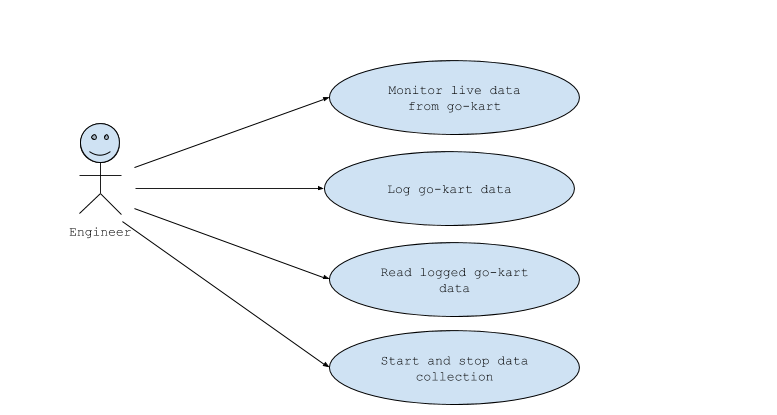
\includegraphics[width=1\textwidth]{graphics/use_cases}
    \caption{Use case diagram for the system.}
    \label{fig:usecases}
\end{figure}

As the goal of this system is to ease development on the go-kart, it should not only ease data collection, but also allow for simple addition of new sensors or other equipment.
Different projects may also have different requirements in terms of the presentation of data.
For this reason it should be possible to add a custom (G)UI of the projects design.
These requirements introduces a distinction between the actors expected to work with the system, the user and the developer.
The user will use the system to extract data from the system.
The developer will work on integrating new data producers into the system.
A use case narrative for each of the use cases is shown in appendix \ref{app:usecase}.
\newpage
%!TEX root = ../main.tex
\begin{thebibliography}{11} %This number should be higher than the number of entries in the bibliography because reasons...
%	\bibitem{id}
%		Author(s) Last name, First name, Company/Organisation, Year. Full Title
	\bibitem{xcanps}
			https://github.com/Xilinx/embeddedsw/blob/master/XilinxProcessorIPLib/drivers/canps/examples/xcanps\_polled\_example.c
	\bibitem{formulastudent}
			University of Southern Denmark, 2014, http://www.sdu-vikings.dk/
	\bibitem{ath9k}
			Open source, June 2015, https://wireless.wiki.kernel.org/en/users/drivers/ath9k\_htc/devices
	\bibitem{boostchat}
			www.boost.org, Boost C++ Libraries, http://www.boost.org/doc/libs/1\_62\_0/doc/html/boost\_asio/examples/cpp11\_examples.html
	\bibitem{beej}
			Hall, Brian, June 2016, Beej's Guide to Network Programming - Using Internet Sockets.
	\bibitem{CAN_introduction}
			Corrigan, Steve, Texas Instruments, July 2008, Introduction to the Controller Area Network (CAN).
	\bibitem{3.3V_CAN}
			Blackman, Jason and Monroe, Scott, Texas Instruments, January 2013, Overview of 3.3V CAN (Controller Area Network) Transceivers.
	\bibitem{interfacenaming}
			Open source, Nov 2015, Predictable Network Interface Names (https://www.freedesktop.org/wiki/Software/systemd/PredictableNetworkInterfaceNames/)
	\bibitem{xillinux}
			Xillybus LTD, http://xillybus.com/xillinux
	\bibitem{Xilinx_wiki_amp}
			Xilinx wiki Asymmetric Multiprocessing, http://www.wiki.xilinx.com/Multi-OS+Support+(AMP+\%26+Hypervisor)
	\bibitem{Xilinx_wiki_Linux_CAN_driver}
			http://www.wiki.xilinx.com/Linux+CAN+driver
	\bibitem{CANopen_introduction}
			http://www.ni.com/white-paper/14162/en/
	\bibitem{Xilinx_AMP}
			John McDougall, February 14, 2013, XAPP1078 v1.0, Simple AMP Running Linux and Bare-Metal System on Both Zynq SoC Processors, https://www.xilinx.com/support/documentation/application\_notes/xapp1078-amp-linux-bare-metal.pdf
	\bibitem{CAN-Utils}
			CAN-Utils tool, https://github.com/linux-can/can-utils/blob/master/README.md
	\bibitem{vectornav}
			VectorNav, vn-100 library, http://www.vectornav.com/support/downloads
	\bibitem{bluetooth}
			Wikipedia, Bluetooth, https://en.wikipedia.org/wiki/Bluetooth
	\bibitem{wiki_wifi}
			Wikipedia, IEEE\_802.11 , https://en.wikipedia.org/wiki/IEEE\_802.11\#Protocol
\end{thebibliography}
\martin{Check cites, ensure that they adhere to the thing and such}
\newpage
\end{document}

